
% This LaTeX was auto-generated from MATLAB code.
% To make changes, update the MATLAB code and republish this document.

\documentclass{article}
\usepackage{graphicx}
\usepackage{color}

\sloppy
\definecolor{lightgray}{gray}{0.5}
\setlength{\parindent}{0pt}

\begin{document}

    
    
\section*{Zachary Kaplan}

\begin{par}
Math 440 Computational Lab \#1 2/14/19
\end{par} \vspace{1em}
\begin{par}
An online version of this file published to latex can be found at: https://www.overleaf.com/read/zvtjspxrnqkv
\end{par} \vspace{1em}
\begin{par}
\textbf{NOTE}: To render latex from this document locally, please include the         following package dependencies:
\end{par} \vspace{1em}

\begin{verbatim}\usepackage[margin=1in]{geometry}
\usepackage{amsmath}
\usepackage{amssymb}
\usepackage{microtype}\end{verbatim}
    
\subsection*{Contents}

\begin{itemize}
\setlength{\itemsep}{-1ex}
   \item The Model and Discretization
   \item Declaration of Constants
   \item Validation of Implementation
   \item Results - Diffusion Only
   \item Results - Diffusion \& Convection
   \item Implementation of ODE solver
\end{itemize}


\subsection*{The Model and Discretization}

\begin{par}
Consider the differential operator
\end{par} \vspace{1em}
\begin{par}
$$ D_T[\cdot] = -\frac{d}{dz}\left(\kappa \frac{d}{dz}\right)
                +\nu\rho C \frac{d}{dz}
              = -\kappa \frac{d^2}{dz^2} + \nu\rho C \frac{d}{dz}, $$
\end{par} \vspace{1em}
\begin{par}
and the driving function
\end{par} \vspace{1em}
\begin{par}
$$ Q(z) = \begin{cases}
            0 & 0 \le z \le a \\
            Q_0 \cdot \sin\left(\frac{z - a}{z - b}\pi\right)
               & a \le z \le b \\
            0 & b \le z \le L
          \end{cases} \quad \forall z \in [0,L], $$
\end{par} \vspace{1em}
\begin{par}
where $0 \le a \le b \le L$.
\end{par} \vspace{1em}
\begin{par}
We then define the function $T(z)$ as the solution to the below system of a second order differential equation and BCs
\end{par} \vspace{1em}
\begin{par}
$$ \begin{cases}
     D_T[T(z)] = Q(z),\quad \forall z \in [0,L] \\
     T(0) = T_0 \\
     -\kappa \frac{d}{dz} T(L) = k(T(L) - T_{out})
   \end{cases}. $$
\end{par} \vspace{1em}
\begin{par}
In order to solve this system numerically, we'll first discretize the linear differential operator $D_T$ using a fixed width partition of $[0,L]$. Our fixed partition $\mathbf{Z} = \begin{pmatrix}    z_0 = 0 & z_1 = h & \ldots &  z_{N-1} = L-h & z_N = L  \end{pmatrix}^\top $ has $N-1$ interior points and a grid spacing of $h = L/N$. We will define our discretized approximation of $T(z)$ as the vector $\mathbf{T} = \begin{pmatrix}    t_0 \approx T(z_0) & t_1 \approx T(z_1) & \ldots      & t_{N-1} \approx T(z_{N-1}) & t_N \approx T(z_N)  \end{pmatrix}^\top $. Using the centered 3-point stencil for second derivatives, and the cenetered difference stencil for first order dirivatives, it follows trivially that $D_T$ may discretize as
\end{par} \vspace{1em}
\begin{par}
$$ D_T[T] \sim \left[
     -\frac{\kappa}{h^2} \begin{pmatrix}
        1 & -2 &  1 &  0 & 0 & \ldots &  0 \\
        0 &  1 & -2 &  1 & 0 & \ldots &  0 \\
        \vdots &  & \ddots & \ddots & \ddots &  & \vdots \\
        0 & \ldots & 0 &  1 & -2 &  1 &  0 \\
        0 & \ldots & 0 &  0 &  1 & -2 &  1 \end{pmatrix}
     +\frac{\nu\rho C}{2h} \begin{pmatrix}
        1 &  0 & -1 &  0 & 0 & \ldots &  0 \\
        0 &  1 &  0 & -1 & 0 & \ldots &  0 \\
        \vdots &  & \ddots & \ddots & \ddots &  & \vdots \\
        0 & \ldots & 0 &  1 &  0 & -1 &  0 \\
        0 & \ldots & 0 &  0 &  1 &  0 & -1 \end{pmatrix}
     \right] \mathbf{T}. $$
\end{par} \vspace{1em}
\begin{par}
The above approximates the evaluation of $D_T$ on the discrete function $\mathbf{T}$ at the interior points $\{z_1, z_2, \ldots, z_{N-1}\}$. Therefore, the constraints imposed by the ODE $D_T[T] = Q$ can be enforced by setting the above equal to $\begin{pmatrix}Q(z_1) & Q(z_2) & \ldots & Q(z_{N-1})\end{pmatrix}^\top$.
\end{par} \vspace{1em}
\begin{par}
The first boundary condition can be trivially enforced by setting $t_0 = T_0$. The second boundary condition can be discretized using the backward first order finite difference to
\end{par} \vspace{1em}
\begin{par}
$$ \begin{split}
     &-\kappa \frac{t_N - t_{N-1}}{h} = k(t_N - T_{out}) \\
     \implies& \left(\frac{\kappa}{kh} + 1\right)t_N
               - \frac{\kappa}{kh}t_{N-1} = T_{out}.
   \end{split} $$
\end{par} \vspace{1em}
\begin{par}
Combining all of the above into a single matrix system, we get a system of the form $A\mathbf{T} = \mathbf{b}$ where
\end{par} \vspace{1em}
\begin{par}
$$ \begin{split}
A &=
     -\frac{\kappa}{h^2} \begin{pmatrix}
        0 &  0 &  0 &  0 & 0 & \ldots &  0 \\
        1 & -2 &  1 &  0 & 0 & \ldots &  0 \\
        0 &  1 & -2 &  1 & 0 & \ldots &  0 \\
        \vdots &  & \ddots & \ddots & \ddots &  & \vdots \\
        0 & \ldots & 0 &  1 & -2 &  1 &  0 \\
        0 & \ldots & 0 &  0 &  1 & -2 &  1 \\
        0 &  0 &  0 &  0 & 0 & \ldots &  0 \end{pmatrix}
     +\frac{\nu\rho C}{2h} \begin{pmatrix}
        0 &  0 &  0 &  0 & 0 & \ldots &  0 \\
        1 &  0 & -1 &  0 & 0 & \ldots &  0 \\
        0 &  1 &  0 & -1 & 0 & \ldots &  0 \\
        \vdots &  & \ddots & \ddots & \ddots &  & \vdots \\
        0 & \ldots & 0 &  1 &  0 & -1 &  0 \\
        0 & \ldots & 0 &  0 &  1 &  0 & -1 \\
        0 &  0 &  0 &  0 & 0 & \ldots &  0 \end{pmatrix}
     +\begin{pmatrix}
        1 & 0 & \ldots & 0 \\
        0 & 0 & \ldots & 0 \\
        0 & 0 & \ldots & 0 \\
        \vdots & \ddots & \ddots & \vdots \\
        0 & \ldots & 0 & 0 \\
        0 & \ldots & 0 & 0 \\
        0 & \ldots & \frac{\kappa}{kh} + 1 & -\frac{\kappa}{kh}
      \end{pmatrix}, \\
\mathbf{b} &=
     \begin{pmatrix}
        T_0 & Q(z_1) & Q(z_2) & \ldots & Q(z_{N-1}) & T_{out}
     \end{pmatrix}^\top.
\end{split} $$
\end{par} \vspace{1em}
\begin{par}
By substituting $t_0 = T_0$ we can easily eliminate the first row of the above matrices. Similarly by writing the second boundary condition as
\end{par} \vspace{1em}
\begin{par}
$$ t_N = \frac{\kappa}{kh + \kappa}t_{N-1}
         + \frac{kh}{kh + \kappa} T_{out} $$
\end{par} \vspace{1em}
\begin{par}
and substituting this into the equation represented by the second to last row of A
\end{par} \vspace{1em}
\begin{par}
$$ \begin{split}
\left(\frac{\nu\rho C}{2h} - \frac{\kappa}{h^2}\right) t_{N-2}
  + 2\frac{\kappa}{h^2} t_{N-1}
  - \left(\frac{\nu\rho C}{2h} + \frac{\kappa}{h^2}\right) t_N
  &= Q(z_{N-1}) \\
\implies \left(\frac{\nu\rho C}{2h} - \frac{\kappa}{h^2}\right) t_{N-2}
  + \left[
      2\frac{\kappa}{h^2}
      - \left(\frac{\nu\rho C}{2h} + \frac{\kappa}{h^2}\right)
          \frac{\kappa}{kh + \kappa}
    \right] t_{N-1}
  &= Q(z_{N-1})
    + \left(\frac{\nu\rho C}{2h} + \frac{\kappa}{h^2}\right)
       \frac{kh}{kh + \kappa} T_{out},
\end{split} $$
\end{par} \vspace{1em}
\begin{par}
we can eliminate the final row as well. This results in the simplified system $A^*\mathbf{T}^0 = \mathbf{b}^*$ where
\end{par} \vspace{1em}
\begin{par}
$$ \begin{split}
A^* &=
     -\frac{\kappa}{h^2} \begin{pmatrix}
        -2 &  1 &  0 & \ldots &  0 \\
         1 & -2 &  1 & \ldots &  0 \\
        \vdots & \ddots & \ddots & \ddots & \vdots \\
        0 & \ldots & 1 & -2 &  1 \\
        0 & \ldots & 0 &  1 & -2 \end{pmatrix}
     +\frac{\nu\rho C}{2h} \begin{pmatrix}
        0 & -1 &  0 & \ldots &  0 \\
        1 &  0 & -1 & \ldots &  0 \\
        \vdots & \ddots & \ddots & \ddots & \vdots \\
        0 & \ldots &  1 &  0 & -1 \\
        0 & \ldots &  0 &  1 &  0 \end{pmatrix}
     +\begin{pmatrix}
        0 & 0 & \ldots & 0 \\
        0 & 0 & \ldots & 0 \\
        \vdots & \ddots & \ddots & \vdots \\
        0 & \ldots & 0 & 0 \\
        0 & \ldots & 0 & K \\
      \end{pmatrix}, \\
K &= -\left(\frac{\nu\rho C}{2h} + \frac{\kappa}{h^2}\right)
       \frac{\kappa}{kh + \kappa}, \\
\mathbf{b}^* &=
     \begin{pmatrix}
        Q(z_1)
          + T_0\left(\frac{\kappa}{h^2} - \frac{\nu\rho C}{2h} \right) &
        Q(z_2) & \ldots & Q(z_{N-2}) &
        Q(z_{N-1}) - K\frac{kh}{\kappa} T_{out}
     \end{pmatrix}^\top,
\end{split} $$
\end{par} \vspace{1em}
\begin{par}
and $\mathbf{T}^0 =  \begin{pmatrix} t_1 & t_2 & \ldots & t_{N-1} \end{pmatrix}^\top$ are the interior points of $\mathbf{T}$.
\end{par} \vspace{1em}
\begin{par}
Therefore, in the lab below we will construct sparse matrix $A^*$ and vector $\mathbf{b}^*$ and numerically solve for $\mathbf{T}^0$. Then we will augment $\mathbf{T}^0$ by prepending $T_0$ and by appending $\frac{\kappa}{kh + \kappa}t_{N-1} + \frac{kh}{kh + \kappa} T_{out}$.
\end{par} \vspace{1em}


\subsection*{Declaration of Constants}

\begin{par}
Below we define the values of many constants for this lab.
\end{par} \vspace{1em}
\begin{verbatim}
global L a b Q_0 kappa k rho C T_out T_0;
L = 10;                   % Length of the pipe.
a = 1;                    % Beginning position of heat coil.
b = 3;                    % Terminal position of heat coil.
Q_0 = 50;                 % Coefficient of heating function.
kappa = 0.5;              % Coefficient of heat condution.
k = 10;                   % Coefficient of heat convection.
rho = 1;                  % Density of the fluid.
C = 1;                    % Heat capacity of the fluid.
T_out = 300;              % Ambient temperature at z = L.
T_0 = 400;                % Fixed fluid temperature at z = 0.
\end{verbatim}


\subsection*{Validation of Implementation}

\begin{par}
\textbf{NOTE}: In a matlab script, all helper functions must be defined after         the body of the script. Therefore, the implementation details of         constructing $A^*$ and $\mathbf{b}^*$, and then finding         \ensuremath{\backslash}mathbf\{T\} can be found in the final section of this file.
\end{par} \vspace{1em}
\begin{par}
\textbf{TODO}
\end{par} \vspace{1em}


\subsection*{Results - Diffusion Only}

\begin{par}
Here we only consider $\nu = 0$, and numerically solve with granularity $N = 10, 20, 40, 80$.
\end{par} \vspace{1em}
\begin{par}
In the resulting graphs, we can see that \textbf{TODO: analyze + check for err}.
\end{par} \vspace{1em}
\begin{verbatim}
figure;   % New figure.
hold on;  % Allow for multiple plots on the same graph.
nu = 0;   % Set fluid velocity to 0 to eliminate convection.
for N = 10*pow2(0:3)
    [Z, T] = lab1_solve(N, nu);  % Run the solver.
    plot(Z, T, 'DisplayName', sprintf('N = %d', N));  % Plot the result.
end
xlabel('z');  % Label the axes.
ylabel('T');
legend;       % Enable the legend (defaults to DisplayName's).
title(sprintf('Solutions for T where \\nu = %d', nu));  % Put a title.
\end{verbatim}

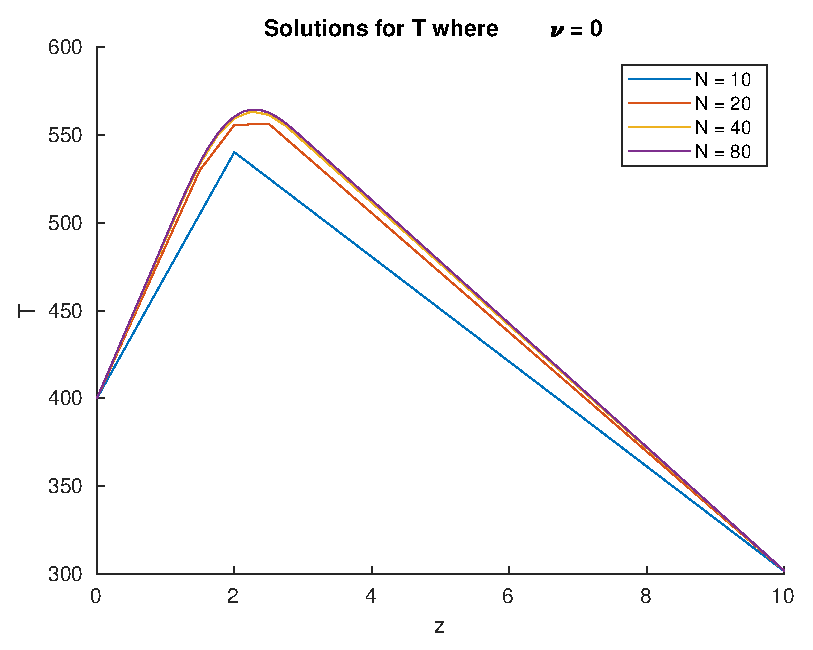
\includegraphics [width=4in]{lab1_01.eps}


\subsection*{Results - Diffusion \& Convection}



\subsection*{Implementation of ODE solver}

\begin{par}
This section contains the implementation of the ODE solver.
\end{par} \vspace{1em}
\begin{verbatim}
function [Z, T] = lab1_solve(N, nu)
% LAB1_SOLVE: solves the linear ODE described in section `The Model and
%             Discretization` above.
%             Parameters:
%               N  - Number of segments to split the interval [0,L] into.
%               nu - Velocity of the fluid through the pipe.
%             Returns:
%               Z  - The N+1 values of [0,L] used in the dicretization.
%               T  - The N+1 approximate evaluations of T(Z).

global L kappa k rho C T_out T_0;

% Partition [0,L].
h = L/N;    % Width of our N intervals.
Z = 0:h:L;  % Discrete support of our solution.

% Coefficients used in matrix A*.
D2_coeff = -kappa/h^2;            % Coefficient of T''(z).
D1_coeff = nu * rho * C / (2*h);  % Coefficient of T'(z).
% Value of constant K that comes up in the second boundary condition.
K = (D2_coeff - D1_coeff) * kappa / (k*h + kappa);

% Linear coefficients of our derivative stencils.
% Here the vectors denote the coefficients along the tri-diagonals of the
% operators: [lower diagonal, major diagonal, upper diagonal].
D2 = [1 -2 1];  % Centered second order FD.
D1 = [1 0 -1];  % Centered first order FD.
DT = D2_coeff * D2 + D1_coeff * D1;  % Our differential operator D_T.

% Construction of matrix A*.
M = N - 1;  % Matrix dimensions of A* in R^{MxM}.
B = ones(M, 1) * DT;  % Columns of length M for the diagonals of A*.
% Account for the boundary conditions.
B(end,2) = B(end,2) + K;  % Add K to the last elem in the major diagonal.
% Construct A* as a sparse MxM matrix with the diagonals specified in B.
% -1:1 denotes the lower, major, and upper diagonals.
Astar = spdiags(B, -1:1, M, M);

% Construction of vector b*$.
bstar = q(Z(2:N)');  % Set b to the evaluation of Q on z_1, ..., z_{N-1}
% Account for the first boundary condition.
bstar(1) = bstar(1) + T_0 * -(D1_coeff + D2_coeff);
% Account for the second boundary condition.
bstar(end) = bstar(end) - K * k * h / kappa * T_out;

% Let T^0 be the solution of A* (.) = b*.
T_interior = Astar \ bstar;

% Add the approximations at the boundaries to T^0.
T = [T_0 ; T_interior ; ...
     (kappa * T_interior(end) + k*h*T_out)/(k*h + kappa)]';

end

function Q = q(Z)
% Q: evaluates the driving heat function described in section `The Model
%    and Discretization` at each point in Z.
%    Parameters:
%      Z - points to evaluate the driving heat function at.
%    Returns:
%      Q - the evaluation of the heat function at each point in Z.

global a b Q_0;

% Logical index representing indices of Z that are inside the heating range
% of the coil.
heating_region = Z > a & Z < b;
% Values of Z in the heating region.
heated_zs = Z(heating_region);

% Create Q as a matrix where the only nonzero elements correspond
% to the values of Z that are in the heating_region.
Q = zeros(size(Z));
Q(heating_region) = Q_0 * sin(pi * (heated_zs - a) ./ (heated_zs - b));

end
\end{verbatim}

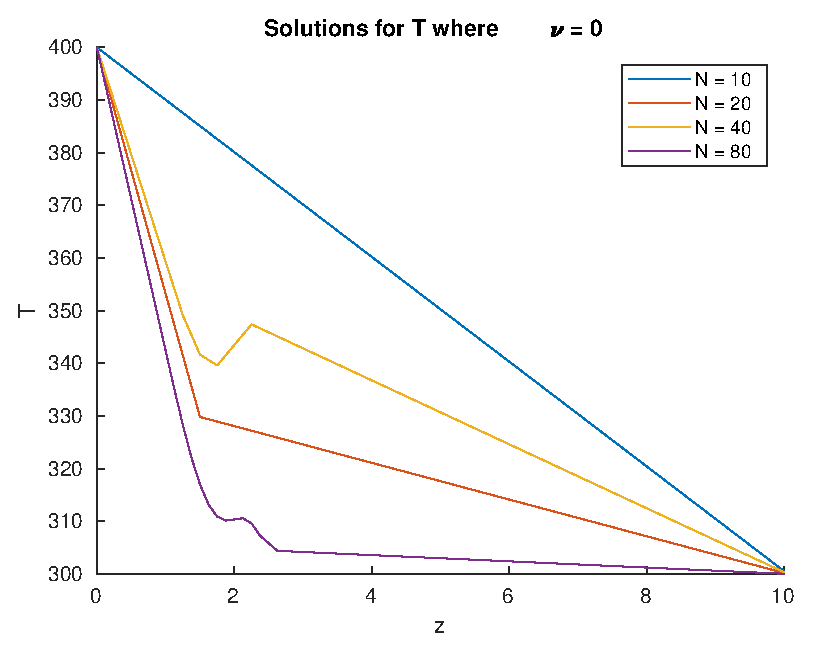
\includegraphics [width=4in]{lab1_02.eps}



\end{document}
    
